\section{Dimensionamento da hélice}

Para o dimensionamento da hélice, inicialmente calculou-se o valor do parâmetro adimensional $j = \frac{V}{nD}$, onde $V$ é a velocidade de cruzeiro, $n$ é a frequência de rotação da hélice e $D$ é o diâmetro. Sabendo que a velocidade da ponta da hélice é dada por
\begin{equation}
V_\text{tip} = \sqrt{(n \pi D)^2+V^2}
\end{equation}
podemos escrever
\begin{equation}
j= \pi\frac{V}{\sqrt{V_\text{tip}-V^2}}
\end{equation}
Considerando que a velocidade da ponta é limitada por perdas de compressibilidade, o número de mach da ponta será limitado a 0,75.

Na condição de cruzeiro, $V=140\si{m/s}$ e a velocidade do som é $a=310\si{m/s}$. O valor de $j$ é então 2,37.

Para obter-se eficiência na faixa de 85\%, selecionou-se uma hélice hexa-pá. De acordo com a \autoref{fig:naca-helice}, a eficiência da hélice para esse valor de $j$ é de 86\% e o coeficiente de tração $T_c = 0,03$. O coeficiente de tração é definido
\begin{equation}
T_c = \frac{\eta P}{\rho D^2 V^3}
\end{equation}
onde $\eta$ é a eficiência da hélice, $P$ é a potência desenvolvida e $D$ é o diâmetro da hélice. Resolvendo essa equação para o diâmetro, temos
\begin{equation}
\label{eqn:D_helice}
D = \sqrt{\frac{\eta P}{\rho V^3 T_c}}
\end{equation}

\begin{figure}[H]
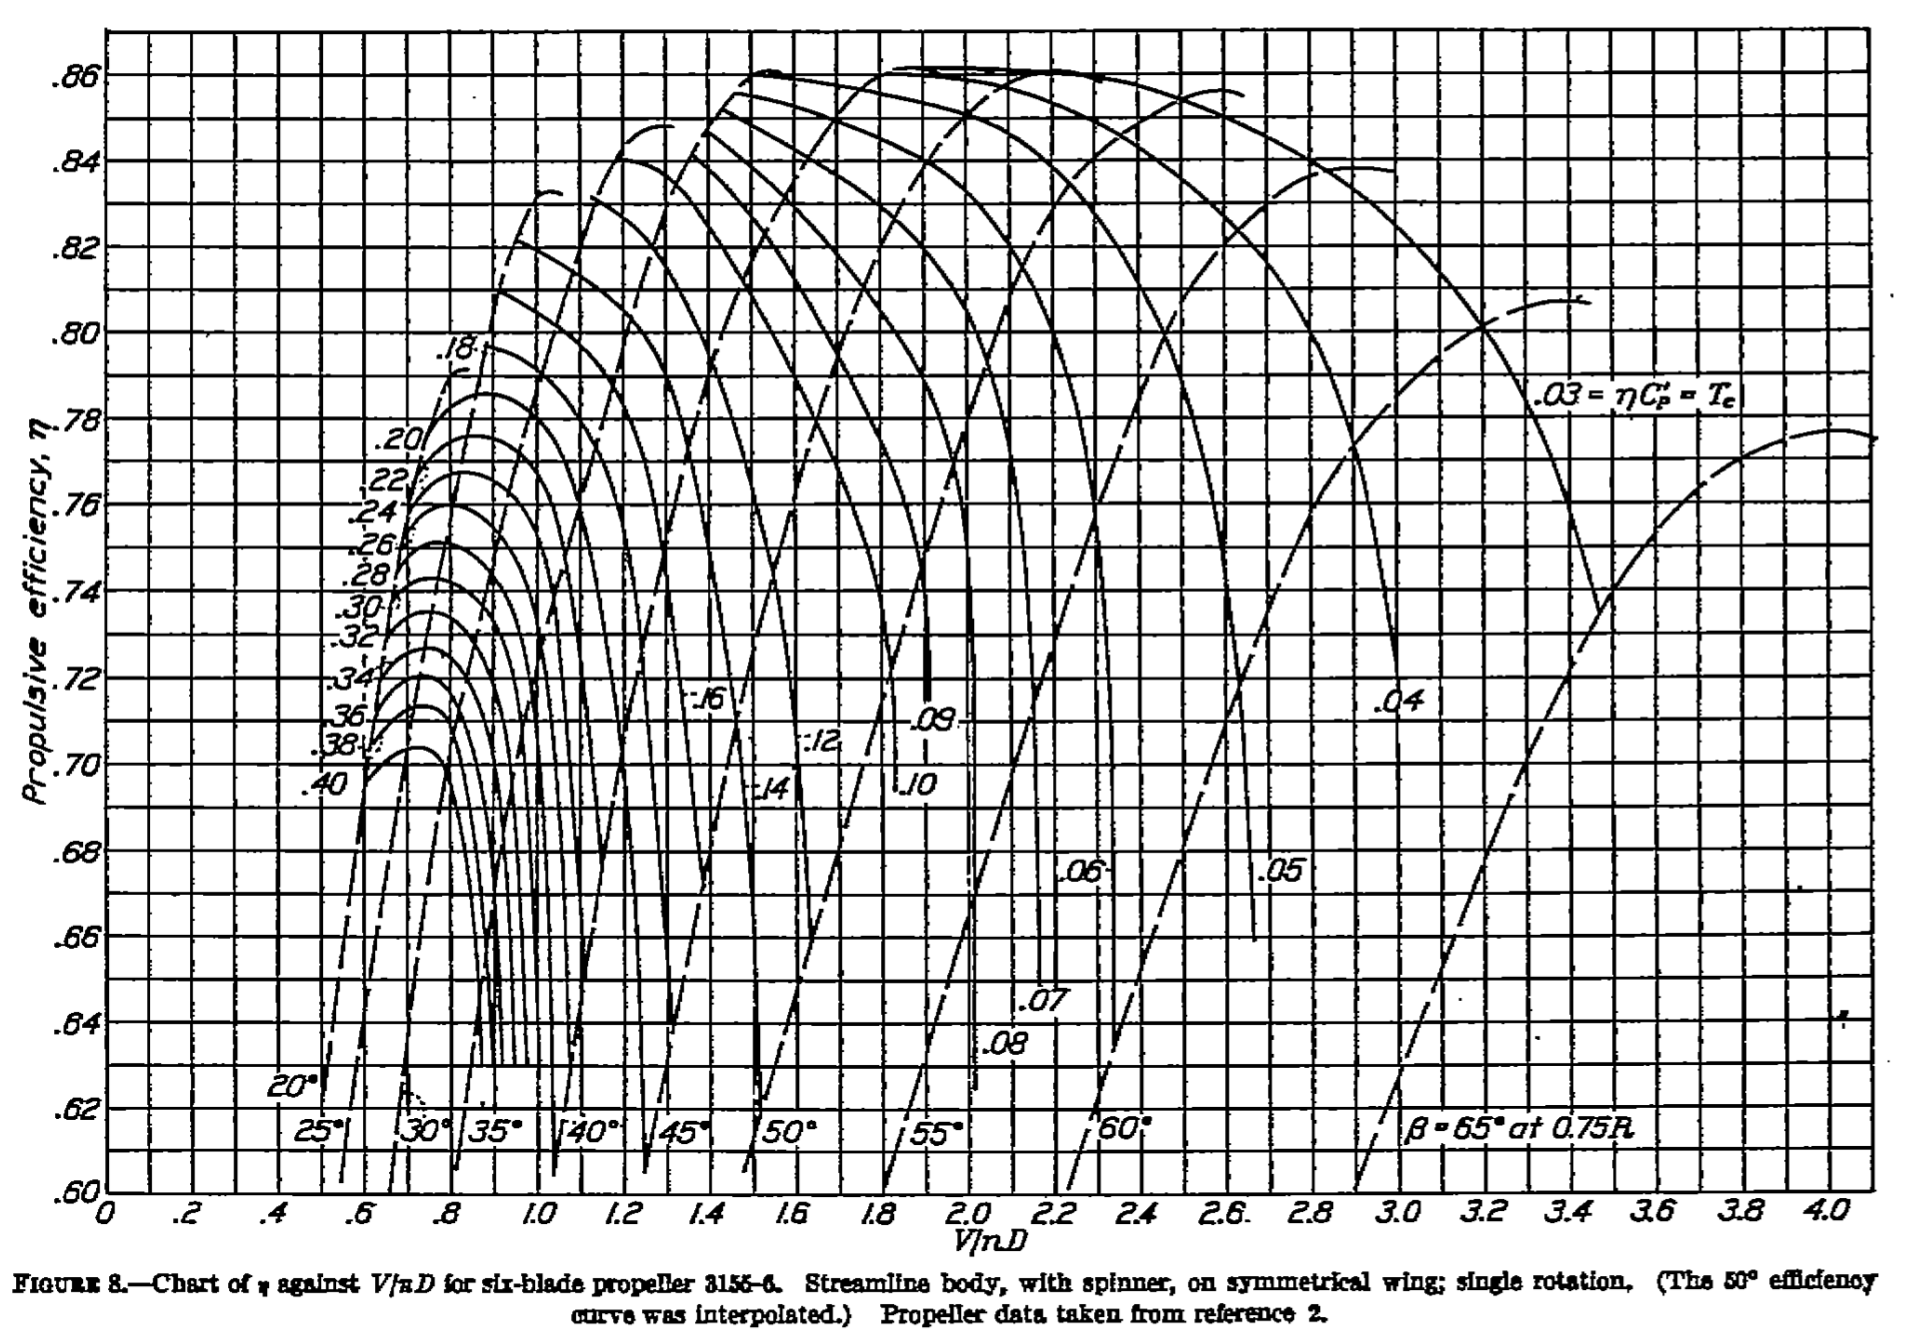
\includegraphics[width=\textwidth]{naca-helice}
\caption{Desempenho de hélice hexa-pá}  % \cite{naca-helice}
\label{fig:naca-helice}
\end{figure}

A potência requerida de decolagem é de 1383\si{kW}, ou seja, 692,5kW por hélice. Substituindo os valores na \autoref{eqn:D_helice}, o diâmetro final fica de
\begin{equation}
D=4,226\si{m}
\end{equation}

Esse diâmetro é aproximadamente duas vezes o diâmetro da fuselagem, de 2,1\si{m}, então não há risco de interferência da hélice com o solo.

%Potencia no cruzeiro: 1383kW (requerida) 2108kW (disponivel) para as duas helices

%Potencia na subida: 3692kW (dimensionante do motor)
